\section{Methods}\label{sec:methods}

I use a mixed-method approach to understanding the inflection of gender through technical documentation. In Section \ref{sec:qual}, I describe the study's methodology in conducting interviews with notable figures from statistical computing in order to understand their conceptualizations of effective documentation, as well as the mechanisms responsible for differences in the way that documentation is structured and presented. Then, in Section \ref{sec:coa}, I describe my methods in conducting a class of object analysis, quantifying these differences in the presentation of code documentation arising from the two development communities described in Section \ref{sec:tidy}.\footnote{The implications of this boundary work delineating between tidyverse and non-tidyverse development are considered more critically in Section \ref{sec:disc}}.

\subsection{Qualitative Interviews}\label{sec:qual}

In order to validate a set of measures attempting to quantify documentation quality, and to more thoroughly investigate the relationship between representation of gender minorities and differences in documentation practices between the tidyverse and other R development communities, I conducted two interviews with women directly involved in this field. Specifically, both of my interviewees hold Ph.D.s in statistics, have taught computational statistics in some setting, and have made significant contributions to the tidyverse, tidyverse-adjacent R packages, or other statistical computing development projects. At the beginning of each interview, I asked for consent to record the interviewee's responses, as well as whether or not they wished to be identified in works resulting from the interviews; one interviewee requested that her responses remain anonymous. Due to the very small size of this sample space, I do not identify either interviewee by name, instead referring to them as interviewee $A$ and $B$. Each interview lasted roughly 30 minutes and was conducted using a semi-structured approach in order to ensure that certain topics were discussed while also allowing for elaboration and clarification on dicussion topics especially relevant to each interviewee. The interview protocol is included in Appendix \ref{sec:interview}.

\subsection{Class of Object Analysis}\label{sec:coa}

Making use of the criteria developed through conducting interviews, I analyze the documentation resources provided alongside software packages on CRAN. Specifically, I examine how the presentation of these resources differs between packages affiliated with the tidyverse (tidy packages) and those not affiliated (non-tidy packages.) R source code for all analyses presented is publicly available online.\footnote{Source code available at: \href{https://github.com/simonpcouch/gendering_documentation}{\textit{https://github.com/simonpcouch/gendering\_documentation}}}


\subsubsection{Data Acquisition} \hspace{10pt} In order to conduct this analysis, I first need to control for factors other than development community that might also contribute to differences in the structure of these resources. Most notably, as my interviewees noted, and as justified in Figure \ref{fig:users}, packages in the tidyverse have, on average, a substantially larger number of monthly downloads than those not in the tidyverse. In order to account for this difference, I use a matched-pairs sampling approach---since there are significantly fewer packages from the tidyverse than from the non-tidy community, I include every tidy package in my sample, and sample the package with the most similar number of package downloads in the last month to each tidy package.\footnote{I do not posit that the actual pairing of these packages is meaningful, but that the overall distribution of usership is important to approximate in order to control for package popularity and, by extension, resources available for maintenance and documentation improvement.}

\begin{figure} [!htb]
    \caption{Distribution of Usership by Development Community}
    \centering
    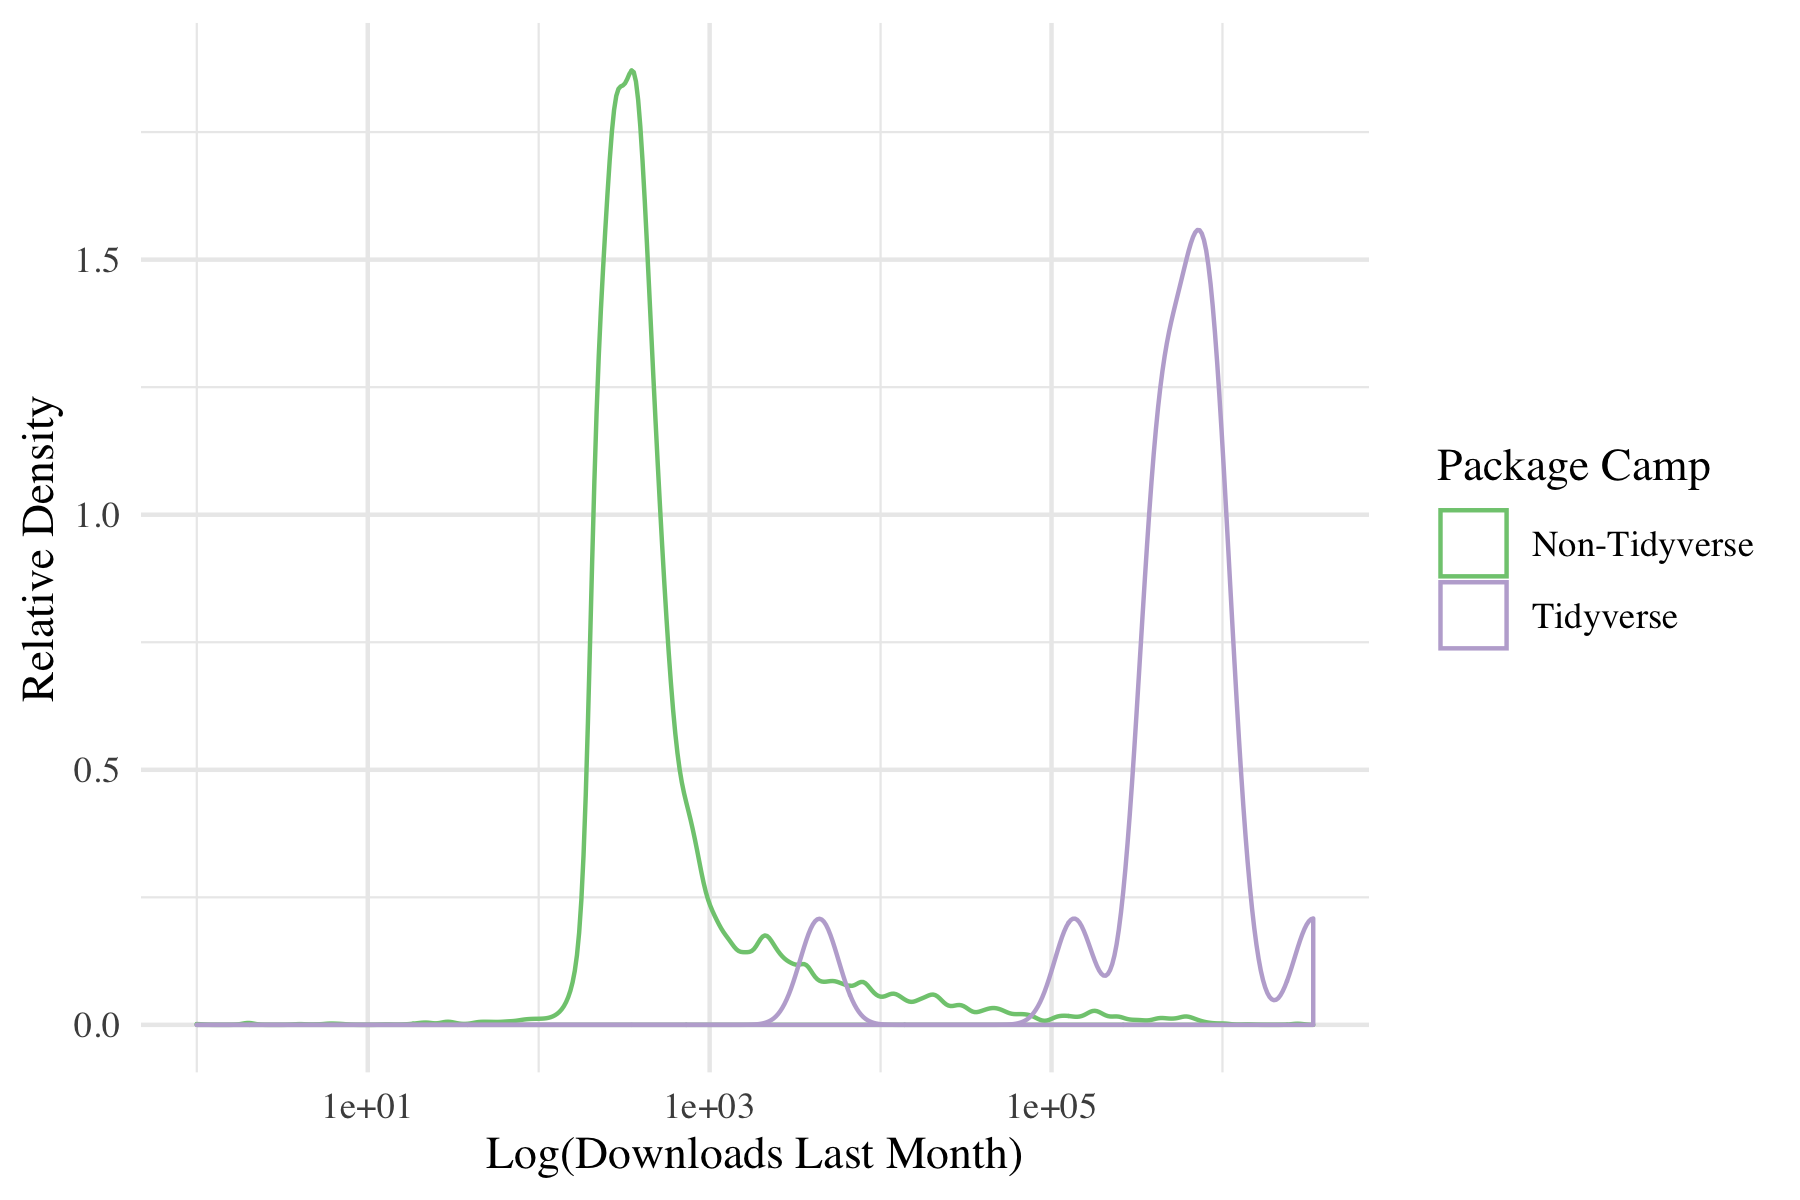
\includegraphics[width=.7\linewidth]{figures/downloads_by_camp.png}
    \captionsetup{width=0.8\textwidth}
    \caption*{Relative density of log (base 10) usership of R software packages in the tidyverse (n = 17, $\mu$ = 755,065) and non-tidyverse (n = 15,227, $\mu$ = 6868).}
    \label{fig:users}
\end{figure}

With this sample of 17 packages from each development community, I then take a census of all exported functions (i.e. those that are available to users) in the packages. In total, this sample includes over 2,200 functions, with 1,500 exported from one of the 17 tidy packages. I then pass each of these functions through an algorithm that extracts variables of interest, described in the next subsection, from the relevant help-files.

\subsubsection{Analysis} \label{sec:met-analyze} \hspace{10pt} The data is collected at the package-level and function-level. My choices of measures to extract from this documentation are a result of my interviews---I've summarized the justification for each of these choices below, alongside discussion from my interviewees.

For package-level documentation, I collect data on two outcomes of interest: whether the package has a \textit{master help-file} accessible by the same help syntax used to seek resources about functions and the \textit{number of vignettes} that the package provides. Accessible master help-files provide a brief introduction into the motivations for using a package, the language and common principles utilized throughout, and directions to find more information on its usage and authorship. Interviewee $A$ started off her answer, when asked about practices for effective documentation, by saying ``one of my pet peeves is packages that don’t have overall documentation.'' Supporting the utilization of my first measure, this interviewee emphasizes the importance of ``providing a general roadmap of what the package is for.'' In regard to my second measure, vignettes are ``a long-form guide to [a] package... [that] can describe the problem that [a] package is designed to solve, and then show the reader how to solve it'' \cite{wickham2015r}. Interviewee $A$ argued that ``multiple types of documentation are very helpful,'' in that the format that works for one learner may be different for another. While this interviewee argued that ``in this day and age, when people want to figure out how to do something, I think they’re a bit more used to clicking around a website'' than reading through plain-text help-files, interviewee $B$ similarly noted that ``the concept of the vignette was really important for making packages more accessible.'' Both of these resources provide a higher-level and more accessible introduction to a package, and the availability of these resources is highly consequential for user understanding.

An arguably greater share of user interaction with documentation happens at the function level. By executing \texttt{?function-name} in the console, users can interact with a relatively standardized, function-specific document (a \textit{help-file}) that describes the purpose of the function, format of user inputs, related functions, and examples. These documents are minimally formatted, containing largely plain text, aside from bolded section headings and links to related help-files. An example help-file is shown in Appendix \ref{fig:ex-help}. While the structure of these help-files is relatively consistent across packages, the amount of content included in these sections, as well as the relative proportion of content devoted to each subsection, varies greatly. Specifically, in my analysis, I focus on the \textit{total character count}, \textit{number of examples}, \textit{number of comments explaining examples}, and \textit{number of functions per help-file}. Interviewee $B$ argued that ``it's really important that you include enough text to actually explain what the function is for and how it's used.'' While basic syntax makes up some portion of the total character count in a help-file, the presence of exposition drastically inflates this number. In general, then, I assert that a greater character count implies a more substantial explanation of functionality and usage and is one useful measure of documentation completeness. While the structure of these help-files is largely standardized, there is significant variation in the number of examples. Examples offer concrete demonstrations of function usage, and are an important element developing a more complete understanding of a function's usage. Interviewee $A$ stated that ``good examples that don’t require domain knowledge or familiarity with a specific dataset'' are an important element of function-level documentation. Further, these examples allow for comments intended to explain the reasoning and intuition behind decisions made within the examples. Interviewee $B$ argued that comments explaining examples are necessary in order to ``make writing any examples worth [the developers'] time." I thus posit that these comments are another important indicator for accessibility and effectiveness of help-files. Finally, while help-files are function-specific in the sense that they can only be evoked using specific functions, several closely-related functions can share one help-file. Interviewee B argued that ``linking between functions [within documentation] is another way'' to make code libraries more accessible. I thus assert that effective documentation elicits the interconnections between functions, and thus that related functions ought to be embedded within the same help-file when applicable.

Based on the differences in representation of gender minorities within the tidyverse and non-tidy development communities and the supply-side mechanisms of gendered occupational segregation described in Section \ref{sec:scholarly}, I present the following hypotheses. Initially, as for package level documentation,

\begin{itemize}
	\item \textit{Hypothesis 1(a):} A larger proportion of packages will provide master help-file in tidy packages than in non-tidy packages.
	\item \textit{Hypothesis 1(b):} Tidy packages will provide a greater mean number of vignettes than non-tidy packages.\footnote{It is important to note here that vignettes were developed as part of the tidyverse ecosystem. An additional mechanism alternative to gender (or gender-conscious) representation within the development community might be that tidy packages are more likely to incorporate this form of documentation due to institutional affiliation.}
\end{itemize}

As for function-level documentation,

\begin{itemize}
	\item \textit{Hypothesis 2(a):} The mean character count of function help-files from tidy packages will be greater than that from non-tidy packages.
	\item \textit{Hypothesis 2(b):} The mean number of examples in function help-files from tidy packages will be greater than that from non-tidy packages.
	\item \textit{Hypothesis 2(c):} The mean number of comments explaining examples in function help-files from tidy packages will be greater than that from non-tidy packages.
	\item \textit{Hypothesis 2(d):} The mean number of functions per help-file will be greater for documentation from tidy packages than that from non-tidy packages.
\end{itemize}

In carrying out significance tests, I use a two-sided significance level $\alpha = .05$.

These hypotheses do not necessarily assert causality related to gender representation. Instead, I intend to argue that documentation practices and gender representation are in constant dialogue. In one way, effectively (and by extension, inclusively) written documentation contributes to an alleviation of the supply side mechanisms discouraging gender minorities' ``self-selection'' away from statistical computing in the tidyverse. Conversely, the greater representation of gender minorities in the tidyverse development community, who are more likely to have encountered documentation written with inclusivity in mind, normalizes and solidifies the expectation of effective and inclusive documentation practices. While the class of object analysis serves only to establish these correlations quantitatively, I explore the arguments for the mechanisms driving them more thoroughly in Section \ref{sec:qual} and \ref{sec:disc}.

